\section{Anhang}
\label{sec:Anhang}


\subsection{Beispiel einer Google Street View Ansicht}
\label{sec:BeispielEinerGoogleStreetViewAnsicht}

\begin{figure}[htb]
\centering
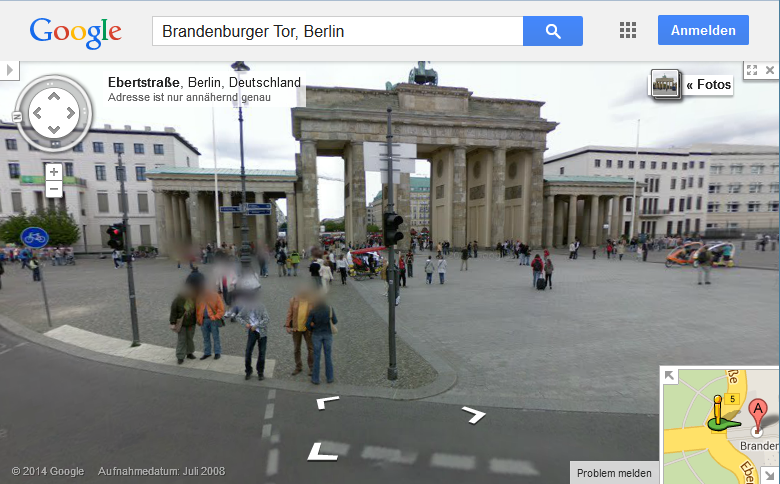
\includegraphics[width=0.7\textwidth]{GoogleStreetView.png}
\caption[Google Street View Beispiel]{Google Street View Beispiel\protect\footnotemark}
\label{fig:GoogleStreetViewBeispiel}
\end{figure}
\footnotetext{Screenshot von \url{https://maps.google.de/}}


\subsection{Javascript-Datei des Prototypen}
\label{sec:AnhangJavascriptPrototyp}

\lstinputlisting[language=JavaScript,caption={Javascript-Datei des Prototypen},label={lst:Javascript Prototyp}]{Listings/JS_Prototyp.js}


\subsection{Bildschirmfoto der Infotextverwaltung}
\label{sec:BildschirmfotoInfotextverwaltung}

\begin{figure}[htb]
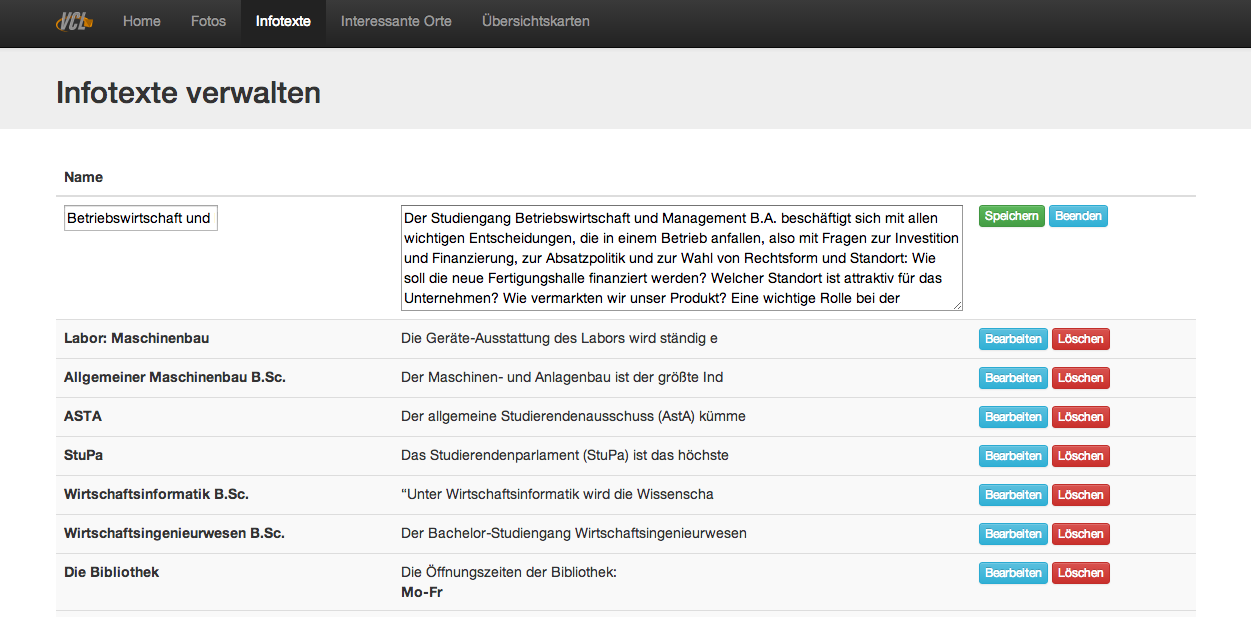
\includegraphics[width=1.0\textwidth]{ScreenshotInfotext.png}
\caption[Bildschirmfoto Infotexte]{Bildschirmfoto der implementierten Infotextverwaltung}
\label{fig:ScreenshotInfotext}
\end{figure}
\centering

\subsection{Bildschirmfoto der Übersichtskarte}
\label{sec:BildschirmfotoUebersichtskarte}

\begin{figure}[htb]
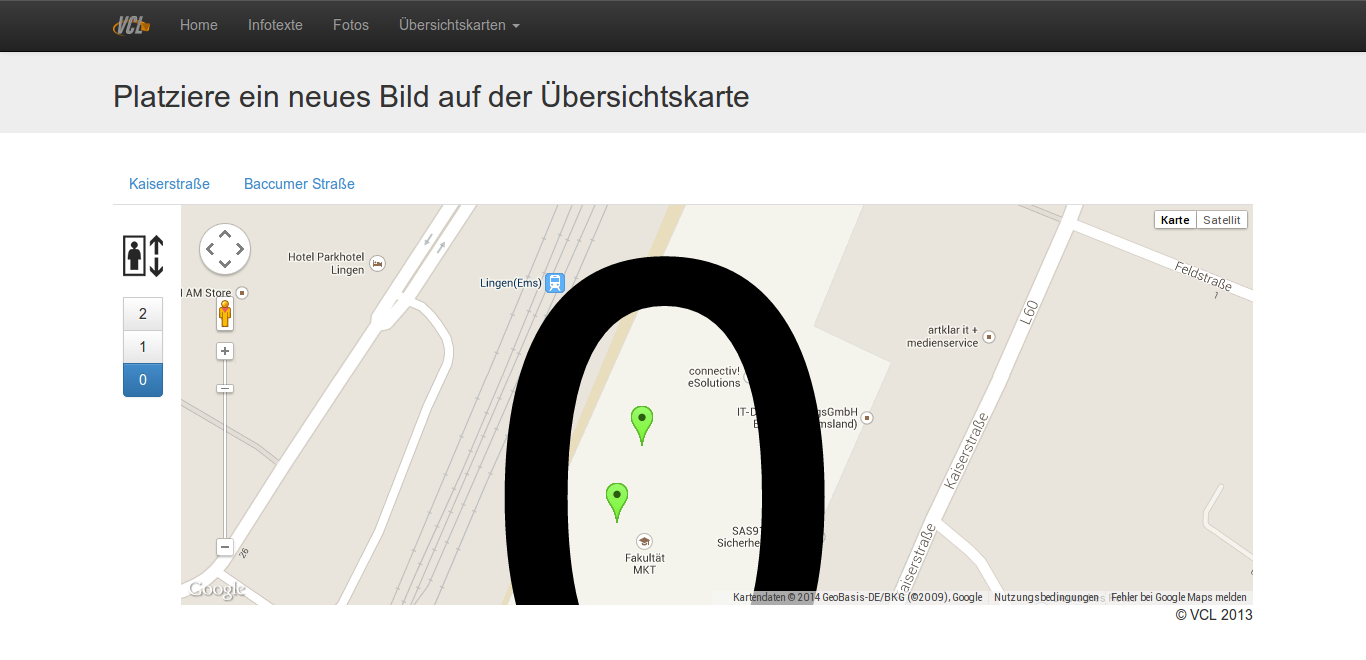
\includegraphics[width=1.0\textwidth]{ScreenshotUebersichtskarte.png}
\caption[Bildschirmfoto Übersichtskarte]{Bildschirmfoto der implementierten Übersichtskarte}
\label{fig:ScreenshotUebersichtskarte}
\end{figure}
\centering